\newsection

\subsection{BP 9:
 Okushiri Island (Field)}

{\bf Documentation:}
\item PMEL-135, pp 8 \& 48-53 \cite{SynolakisBernard:pmel135}.
\item A problem description is provided by Frank Gonz\'alez 
 at \cite{bp-description}:\\
\href{https://github.com/rjleveque/nthmp-benchmark-problems/blob/master/BP09-FrankG-Okushiri_island/Description.pdf} 
\item Numerous other publications also describe this event, in varying detail: \cite{DCRC1994, HTSG1993, KatoTsuji1994, TakahashiEtAl1995, Takahashi1996}
\end{itemize} 

\subsubsection{Description}
The goal of this Benchmark Problem (BP) is to compare computed model results with field observations of the 1993 Okushiri Island tsunami.

\subsubsection {Problems encountered}

\begin {itemize}
\item The primary problem encountered was the uncertain quality of the computational bathymetric topographic grids. 

\end{itemize} 

\subsubsection{What we did}

\begin{itemize}
\item Used g = 9.81 and no friction.
\item Used bathy/topo grids and source grid for the Disaster Control Research Center solution DCRC17a.  Dmitry Nicolsky provided improved versions of the originals developed by Kansai University, in which severe misalignments in the original data were reduced.  The computational domain and initial conditions imposed by the source deformation are presented in Figure \ref{DomainSource}
\end{itemize}

\begin{figure}[ht]
\hfil\includegraphics[width=6.0in]{bp9/DomainSource.png}\hfil
\caption{\label{DomainSource}
Computational domain and source deformation.
  }
\end{figure} 

\subsubsection{Problem Requirements}
  Requirements of this benchmark test were to:
\begin{itemize}
\item 1. Compute runup around Aonae
\item 2. Compute arrival of the first wave to Aonae
\item 3. Show two waves at Aonae approximately 10 min apart; the first wave came from the west, the second wave came from the east
\item 4. Compute water level at Iwanai and Esashi tide gauges
\item 5. Maximum modeled runup distribution around Okushiri Island
\item 6. Modeled runup height at Hamatsumae
\item 7. Modeled runup height at a valley north of Monai
\end{itemize}

\subsubsection{Results}

  Arrival of the first wave at Aonae (Requirement 2) is shown in Figure \ref{AonaeFirstWave} and the subsequrent runup around Aonae (Requirement 1) is presented in Figure \ref{AonaeRunup}.  The first wave arrived at about t = 5 minutes, and wrapped around the peninsula, engulfing Aonae proper in about 2 minutes, at t = 7 minutes, as seen in Figure \ref{Aonae07min.png}.  Between 9 and 10 minutes later, at t=16 and 17 minutes, Hamatsumae (\ref{Aonae16min.png} and then the northeastern coast of the Aonae peninsula \ref{Aonae17min.png} are inundated by a wave from the east (Requirements 3 and 6).  Figures \ref{WestObsVsGeoClaw} and \ref{EastObsVsGeoClaw} present the observed and modeled maximum runup distribution on the West and East coasts of Okushiri, respectively (Requirement 5), including a valley north of Monai where the observed runup height that exceeded 30 m \ref{WestObsVsGeoClaw} (Requirement 7).  Figures \ref{Iwanai} and \ref{Esashi} present the model results and tide gage time series at Iwanai and Esashi.  The correspondence of model and observed tides is poor at both locations, perhaps due to the issue of inaccurate spatial registration of the tide gage positions and the corresponding computational grid cell.  

 Computed arrival times agree well with eye-witness observations at Aonae and Hamatsumae, and computed runup values agree reasonably well with observed values (Figure \ref{WestObsVsGeoClaw}).  


\begin{figure}[ht]
\hfil\includegraphics[width=5.0in]{bp9/AonaeFirstWave.png}\hfil
\caption{\label{AonaeFirstWave}
First wave arrival at Aonae.
  }
\end{figure} 

\begin{figure}[ht]
\hfil\includegraphics[width=5.0in]{bp9/Aonae07min.png}\hfil
\caption{\label{Aonae07min}
Runup at Aonae.
  }
\end{figure}

\begin{figure}[ht]
\hfil\includegraphics[width=5.0in]{bp9/Aonae16min.png}\hfil
\caption{\label{Aonae16min}
Second wave from the east begins to inundate Hamatsumae and the northeastern coast of the Aonae peninsula.
  }
\end{figure} 

\begin{figure}[ht]
\hfil\includegraphics[width=5.0in]{bp9/Aonae17min.png}\hfil
\caption{\label{Aonae17min}
Runup at Hamatsumae and the northeastern coast of the Aonae peninsula.
  }
\end{figure} 

\begin{figure}[ht]
\hfil\includegraphics[width=5.0in]{bp9/WestObsVsGeoClaw.pdf}\hfil
\caption{\label{WestObsVsGeoClaw}
Observed and modeled maximum runup on the Okushiri West Coast.
  }
\end{figure} 

\begin{figure}[ht]
\hfil\includegraphics[width=5.0in]{bp9/EastObsVsGeoClaw.pdf}\hfil
\caption{\label{EastObsVsGeoClaw}
Observed and modeled maximum runup on the Okushiri East Coast.
  }
\end{figure} 

\begin{figure}[ht]
\hfil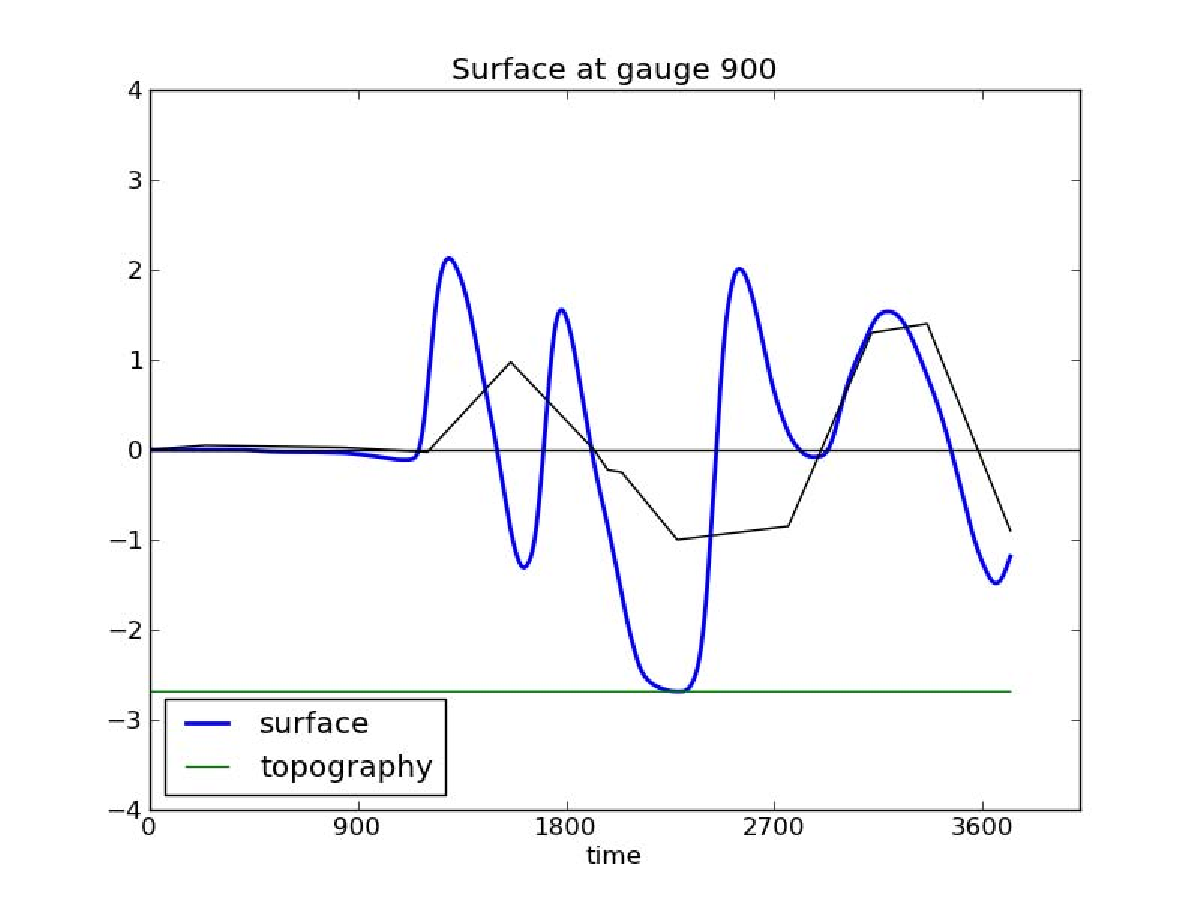
\includegraphics[width=5.0in]{bp9/Iwanai.pdf}\hfil
\caption{\label{Iwanai}
Iwanai tide gage (black line) and GeoClaw (blue line) time series. 
  }
\end{figure}

\begin{figure}[ht]
\hfil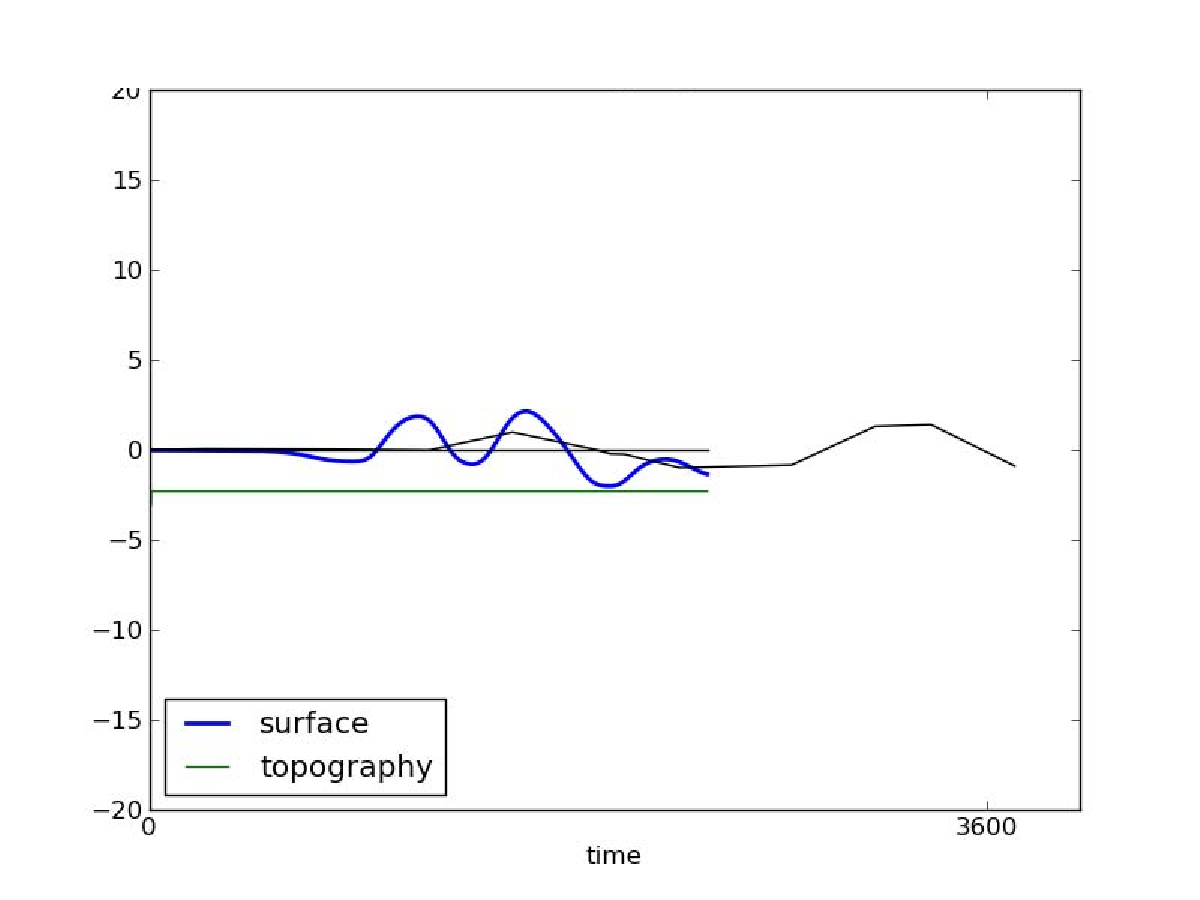
\includegraphics[width=5.0in]{bp9/Esashi.pdf}\hfil
\caption{\label{Esashi}
Esashi tide gage (black line) and GeoClaw (blue line) time series. 
  }
\end{figure}

\subsubsection{Lessons learned}
\begin{itemize}
\item This BenchMark problem requires much more work to qualify as a credible test of tsunami inundation models.  We have little confidence in 
   1. The quality of the bathy/topo computational grids.  A number of mismatches and discontinuities still exist in the system of grids.  A critical related issue is ... 
   2. The accuracy of geospatial registrations of observational and computational latitude and longitude values.  As one example, there appear to be discrepancies in the several field team reports of the latitude and longitude of the highest runup observed, i.e., the value of over 30 m in a " ... small valley north of Monai ...".  Figure \ref{TeamStations} presents the observation locations of each of three field survey teams -- Professor Yoshinobu Tsuji, Tokyo University (Tsuji), the United States-Japan Cooperative Program on Natural Resources (UJNR) and the Tohoku University (Tohoku) teams.  The bathy/topo computational grids were adjusted to match the positions of the Tsuji observations, but it is clear that this created a systematic error in the registration of the grids with the Tohoku field observations and, in all likelihood, the UJNR field observations.  Such positioning errors can be critical with respect to accurate comparisons of observed and computed runup.
\end{itemize}

\begin{figure}[ht]
\hfil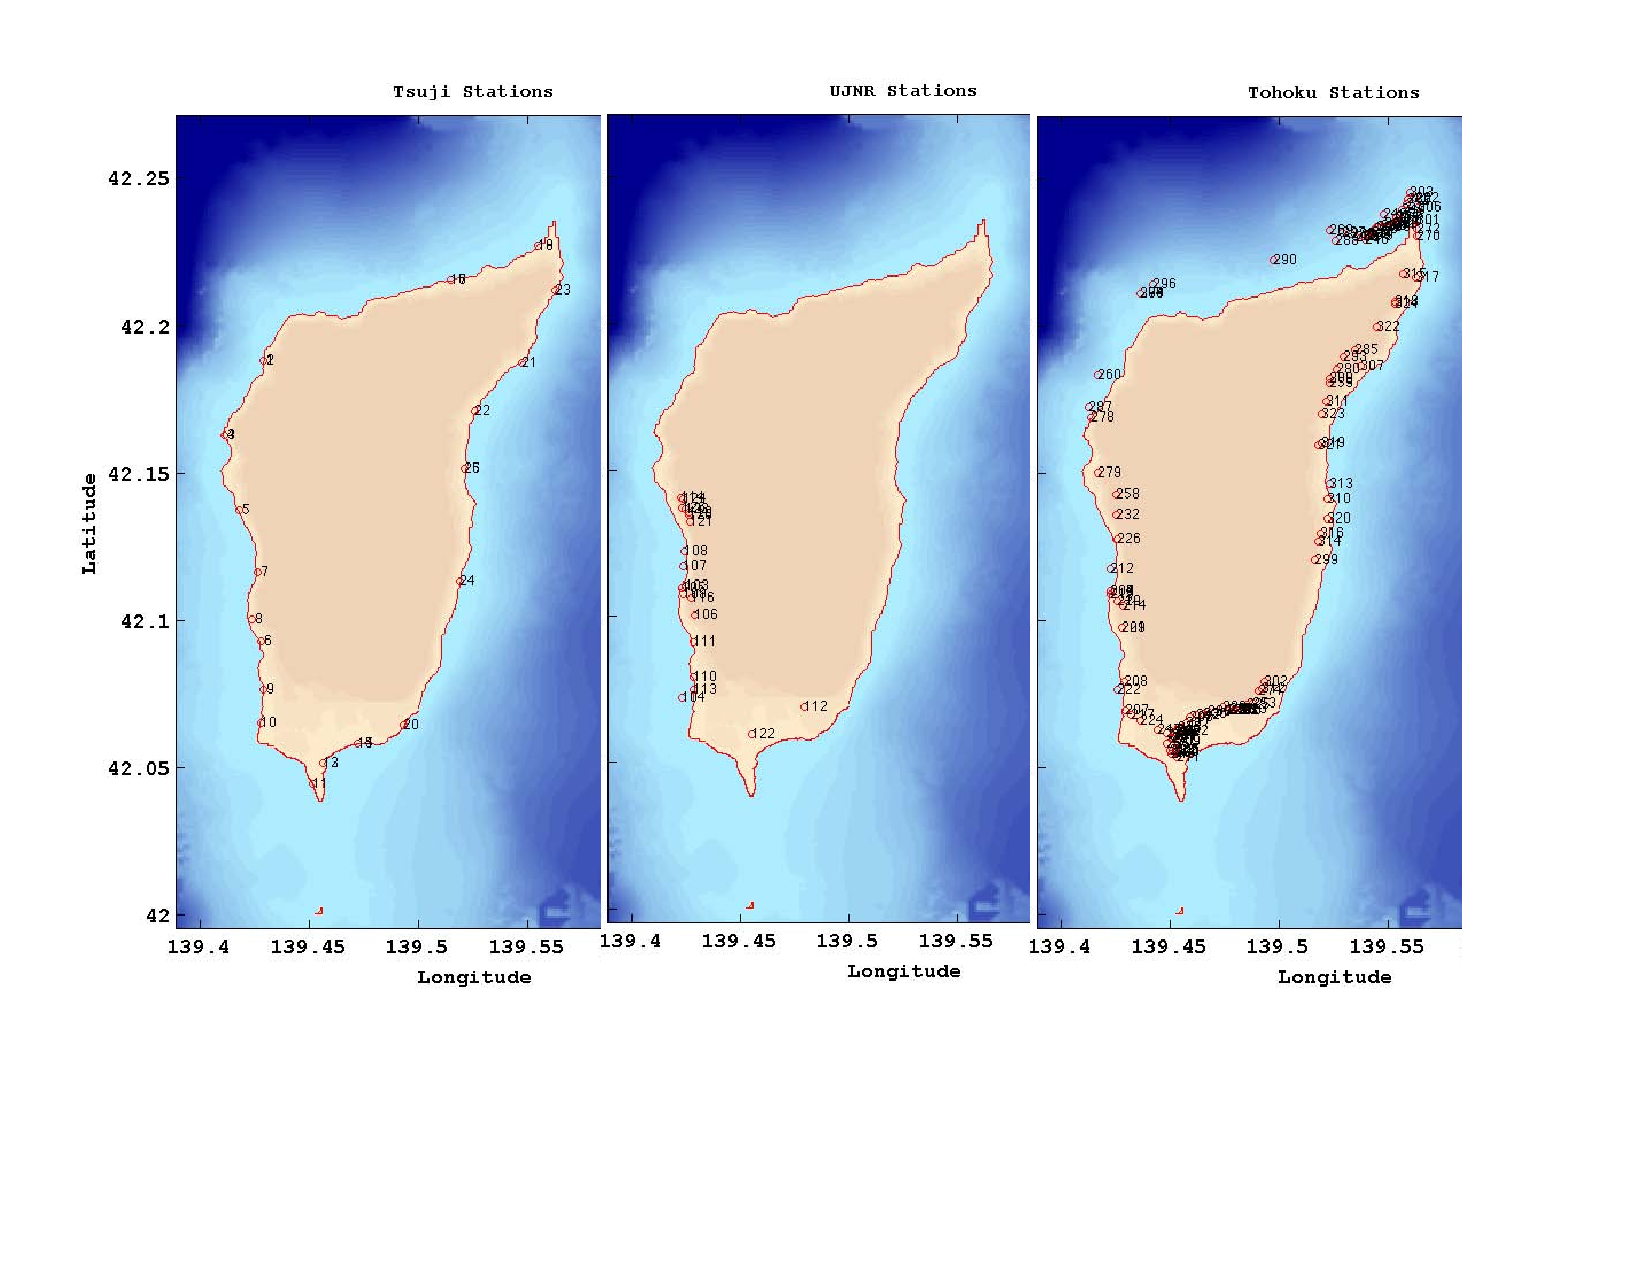
\includegraphics[width=5.0in]{bp9/TeamStations.pdf}\hfil
\caption{\label{TeamStations}
Locations of field observations by three independent field survey teams, relative to the computational bathy/topo grid system. 
  }
\end{figure}

\subsubsection{Recommendation}
\begin{itemize}
\item In spite of the currently low quality state of this benchmark problem, the Okushiri tsunami runup and eyewitness observations remains one of the most valuable datasets for model comparisons in existence.  We recommend that an effort be supported to (a) provide a high quality bathy/topo grid system, (b) resolve the ambiguities and discrepancies currently found in the various team data reports to improve the geospatial registration of observed and modeled values, and (c) provide adequate documentation of the resulting benchmark problem dataset.
\end{itemize}



\begin{itemize}
\item 
\end{itemize}